\documentclass{ximera}

\newcommand{\RR}{\mathbb R}
\renewcommand{\d}{\,d}
\newcommand{\dd}[2][]{\frac{d #1}{d #2}}
\renewcommand{\l}{\ell}
\newcommand{\ddx}{\frac{d}{dx}}
\newcommand{\dfn}{\textbf}
\newcommand{\eval}[1]{\bigg[ #1 \bigg]}


\title[Dig-In:]{Differentiability implies continuity}

\begin{document}
\begin{abstract}
\end{abstract}
\maketitle

As you may have guessed, there is some connection to continuity and
differentiability. 



\begin{theorem}[Differentiability Implies Continuity]\label{theorem:diff-cont}
If $f(x)$ is a differentiable function at $x = a$, then $f(x)$ is
continuous at $x=a$.
\end{theorem}

\begin{proof}
We want to show that $f(x)$ is continuous at $x=a$, hence we must show that 
\[
\lim_{x\to a} f(x) = f(a).
\]
Consider
\begin{align*}
\lim_{x\to a} \left(f(x) - f(a)\right) &= \lim_{x\to a} \left((x-a)\frac{f(x) - f(a)}{x-a}\right) &\text{Multiply and divide by $(x-a)$.} \\
&= \lim_{h\to 0} h \cdot \frac{f(a+h) - f(a)}{h} &\text{Set $x = a+h$.} \\
&= \left(\lim_{h\to 0} h\right) \left(\lim_{h\to 0}\frac{f(a+h) - f(a)}{h}\right) &\text{Limit Law.} \\
&= 0\cdot f'(a) = 0.
\end{align*}
Since 
\[
\lim_{x\to a}\left(f(x) - f(a)\right) = 0 
\]
we see that $\lim_{x\to a} f(x) = f(a)$, and so $f(x)$ is continuous.
\end{proof}

This theorem is often written as its contrapositive:
\begin{quote}
If $f(x)$ is not continuous at $x=a$, then $f(x)$ is not
differentiable at $x=a$.
\end{quote}


Let's see a function that is continuous whose derivative does not
exist everywhere.


\begin{example}
Compute 
\[
\ddx |x|.
\]
\end{example}
\begin{image}
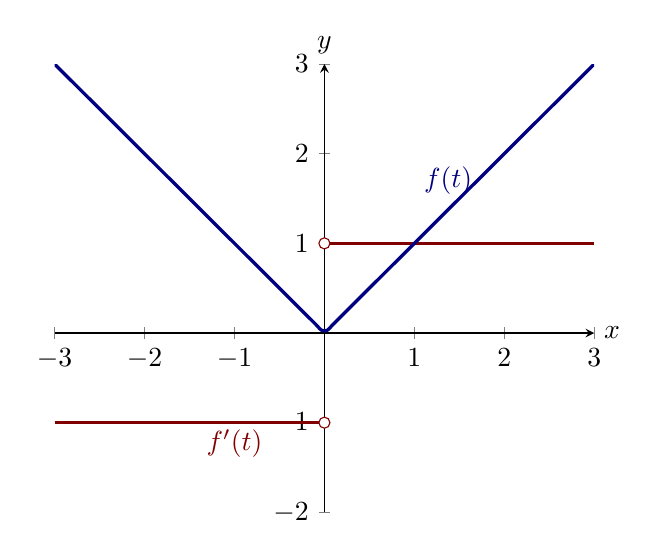
\begin{tikzpicture}
  \colorlet{penColor}{blue!50!black}
  \colorlet{penColor2}{red!50!black}
  \colorlet{textColor}{black}
  \colorlet{background}{white}
	\begin{axis}[
            domain=-3:3,
            ymax=3,
            ymin=-2,
            samples=100,
            axis lines =middle, xlabel=$x$, ylabel=$y$,
            every axis y label/.style={at=(current axis.above origin),anchor=south},
            every axis x label/.style={at=(current axis.right of origin),anchor=west}
          ]
          \addplot [very thick, penColor2, smooth,domain=(0:3)] {1};
          \addplot [very thick, penColor2, smooth,domain=(-3:0)] {-1};
          \addplot [very thick, penColor, smooth] {abs(x)};
          \node at (axis cs:1,1.7) [anchor=west] {\color{penColor}$f(t)$}; 
          \node at (axis cs:-1,-1.5) [anchor=south] {\color{penColor2}$f'(t)$};
          \addplot[color=penColor2,fill=background,only marks,mark=*] coordinates{(0,1)};  %% open hole
          \addplot[color=penColor2,fill=background,only marks,mark=*] coordinates{(0,-1)};  %% open hole
        \end{axis}
\end{tikzpicture}
%\caption[A plot of $f(x) = |x|$ and its derivative.]{A plot of $f(x) = |x|$ and \[
%f'(x) = \begin{cases}
%1 &\text{if $x>0$,}\\
%-1 &\text{if $x<0$.}
%\end{cases}\]
%}
%\label{figure:plot-abs}
\end{image}
\begin{solution}
Using the definition of the derivative,
\[
\ddx |x| = \lim_{h\to0}\frac{|x+h| -|x|}{h}.
\]
If $x$ is positive we may assume that $x$ is larger than $h$, as we are
taking the limit as $h$ goes to $0$,
\begin{align*}
\lim_{h\to0}\frac{|x+h| -|x|}{h} &= \lim_{h\to0}\frac{x+h -x}{h}\\
&= \lim_{h\to0}\frac{h}{h}\\
&= 1.
\end{align*}
If $x$ is negative we may assume that $|x|$ is larger than $h$, as we are taking
the limit as $h$ goes to $0$,
\begin{align*}
\lim_{h\to0}\frac{|x+h| -|x|}{h} &= \lim_{h\to0}\frac{-x-h +x}{h}\\
&= \lim_{h\to0}\frac{-h}{h}\\
&= -1.
\end{align*}
However we still have one case left, when $x=0$. In this situation, we
must consider the one-sided limits:
\[
\lim_{h\to0+}\frac{|x+h| -|x|}{h}\qquad\text{and}\qquad \lim_{h\to0-}\frac{|x+h| -|x|}{h}.
\]
In the first case, 
\begin{align*}
\lim_{h\to0+}\frac{|x+h| -|x|}{h} &= \lim_{h\to 0+}\frac{0+h - 0}{h}\\
&= \lim_{h\to 0+}\frac{h}{h}\\
&=1.
\end{align*}
On the other hand
\begin{align*}
\lim_{h\to0-}\frac{|x+h| -|x|}{h} &= \lim_{h\to 0-}\frac{|0+h| - 0}{h}\\
&= \lim_{h\to 0-}\frac{|h|}{h}\\
&=-1.
\end{align*}
Hence we see that the derivative is
\[
f'(x) = 
\begin{cases}
1 &\text{if $x>0$,}\\
-1 &\text{if $x<0$.}
\end{cases}
\]
Note this function is undefined at $0$, see Figure~\ref{figure:plot-abs}. 
\end{solution}


Thus from Theorem~\ref{theorem:diff-cont}, we see that all
differentiable functions on $\RR$ are continuous on $\RR$. Nevertheless
as the previous example shows, there are continuous functions on $\RR$
that are not differentiable on $\RR$.

\end{document}
